\documentclass[12pt]{article}
\usepackage[utf8]{inputenc}

\usepackage{fullpage}
\usepackage{graphicx}
\usepackage{amsthm}
\usepackage{tikz}
\usepackage[spanish]{babel}
\usepackage{multirow}
\usepackage{framed}

\newtheorem{definition}{Definición}
\newtheorem{lemma}{Proposición}

\begin{document}
\begin{titlepage}
\begin{center}

\includegraphics[scale=0.2]{logo_upc.png}

\begin{Huge}
Trabajo final: Matem\'{a}tica Discreta
\end{Huge}
\vspace{1.5cm}
\begin{Large}\\
\vspace{0.5cm}
Secci\'{o}n: SI-31 Ciclo: 2017-1\\
\vspace{1.5cm}
Integrantes:\\
\item Agreda, Luis Enrique\\
\item Denegri, Jos\'{e}\\
\item Schialer, Dominic\\
\item Uribe, Antonio\\
\vspace{1.5cm}
Profesor: Medina Martines, Antonio Marcos
\vfill
\today
\end{Large}
\end{center}
\newpage
\tableofcontents
\end{titlepage}
\newpage
\section{Introducci\'{o}n: Los puentes de K\"{o}nigsberg}
\begin{center}
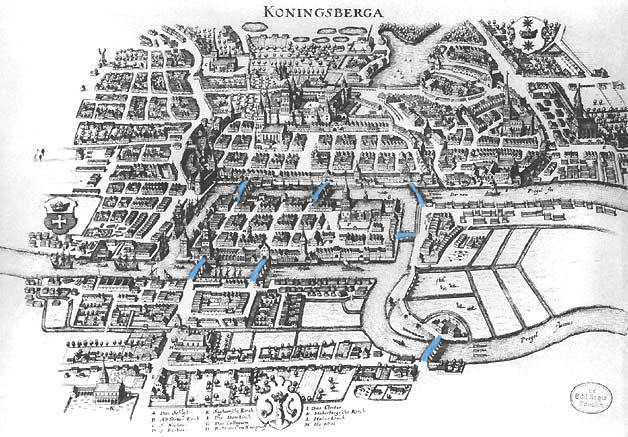
\includegraphics[scale=0.5]{koenigsberg.jpg}
\end{center}
El problema de los puentes de K\"{o}nigsberg ha generado muchas interrogantes en los matemáticos del siglo 18. La meta es de encontrar un camino que vaya por la ciudad, cruzando exactamente una vez cada uno de los siete puentes y terminar el recorrido en el mismo lugar donde comenzó. En 1736 este problema es resuelto por el matemático suizo Leonard Euler, que en ese momento era profesor de matemática en la universidad de San Petersburgo. Euler logró demostrar, que dicho camino no puede existir.\\ Ese descubrimiento estableci\'{o} los fundamentos para la teor\'{i}a de los grafos, que actualmente tiene un sinf\'{i}n de aplicaciones en el mundo real.
\subsection{Euler y el problema de los puentes de K\"{o}nigsberg}
Al buscar un camino cíclico, el cual cruce los siete puentes de K\"{o}nigsberg exactamente una vez, escribe Euler, que una forma de resolver el problema, era trazar todos los caminos posibles y revisar si alguno de ellos tiene las características deseadas. Esta solución es demasiado trabajosa para problemas más complejos, por lo cual Euler quería desarrollar un método matemático que le indique si un camino así sería posible. Primero simplificó el mapa de K\"{o}nigsberg, tal que la secuencia de letras A,B,C y D pueda describir cada camino posible por la ciudad.
\begin{center}
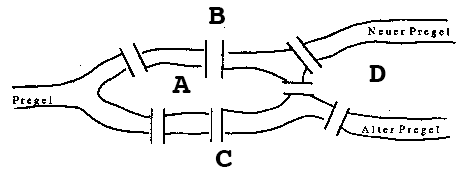
\includegraphics[scale=0.7]{pregelbruecken.png}
\end{center}
Por ejemplo, la secuencia $ADCABAC$ describe el camino que comienza en A, cruza el puente para llegar a $D$, va de $D$ a $C$, etc. Este camino cruza seis de los siete puentes, los cuales pueden ser descritos como los pares $AD$, $DC$, $CA$, $AB$, $BA$ y $AC$. Esto simplifica el problema, ya que solamente se tiene que encontrar una secuencia de 8 letras (ya que se trata de 7 puentes), en la que cada letra aparezca en relación a la cantidad de puentes que la conecta. Antes de buscar esa secuencia, Euler quería demostrar que existe. Euler argumenta que $D$ tiene que aparecer exactamente dos veces en esa secuencia, ya que $D$ está conectado con tres puentes. Si $D$ aparece una vez en la secuencia, solamente se cruzarían dos de los tres puentes. Si $D$ aparece tres veces en la secuencia, debería estar conectado con, como mínimo, cuatro puentes. Asimismo deberían aparecer $C$ y $B$ dos, y $A$ tres veces. Por lo tanto, la secuencia necesitaría 9 letras, lo que es imposible, ya que solamente hay 7 puentes. Esto demuestra que un camino que cruce cada puente un a sola vez y que termine en la letra que comenzó, no existe. 
\section{Objetivo}
El objetivo del siguiente trabajo, es crear un programa que genere un grafo aleatorio de 6 a 12 nodos, cuyos grados sean pares. Luego se simular\'{a} a un cartero que parte de un nodo cualquiera (la oficina del correo) y que tenga que repartir cartas en todas las calles señaladas,  representadas por las aristas del grafo. Para ayudar al cartero, el camino tiene que ser el m\'{a}s corto posible, lo que quiere decir que ninguna de las calles se debe recorrer m\'{a}s de una vez y que al final de su recorrido, llegue de regreso a la oficina del correo. 
\section{Fundamentos te\'{o}ricos}
\subsection{Caminos y grafos eulerianos}
\begin{definition}
Un camino $C$ en un grafo conexo $G$ se le denomina \emph{camino euleriano}, cuando cada arista de $G$ se encuentra en $C$.
\end{definition}
\begin{definition}
Un grafo conexo $G$ se le denomnia \emph{grafo euleriano}, cuando contiene un camino euleriano cerrado. Un camino euleriano cerrado se le llama ciclo euleriano.
\end{definition}
\begin{lemma}
Sea un grafo conexo $G$ con los siguientes atributos:
\begin{enumerate}
\item $G$ es un grafo euleriano.
\item Cada nodo de $G$ tiene un grado par.
\item Las aristas de $G$ se pueden separar en ciclos disjuntos.
\end{enumerate}
\end{lemma}
\begin{proof}
La proposición es demostrada mediante el razonamiento circular.
\\$1. \rightarrow 2.$
\\Asumimos que $G$ contenga un ciclo euleriano $C$. Sea $v$ un nodo cualquiera de $G$. Cada vez que $C$ pase por $v$, tiene que pasar por dos aristas incidentes a $v$. Si cada arista incidente a $v$ es recorrida por $C$, entonces el grado de $v$ es par.
\\$2. \rightarrow 3.$
\\Asumimos que el grado cada nodo $v \in G$ es par. Ya que $G$ es un grafo conexo y ningún nodo tiene un grado de 1, entonces $G$ no es un árbol y, por lo tanto, tiene por lo menos un ciclo. Tiene $G$ exactamente un ciclo, entonces es $G$ un grafo ciclo $C_{n}$ para un $n$ y la disyunción seria solo ese ciclo. Suponiendo que sea verdadero para grafos que no contengan mas de $k$ ciclos y $G$ contiene $k+1$ ciclos. Sea $C$ un ciclo en $G$ y sea $G'$ el grafo resultante de $G$, cuando se eliminan las aristas pertenecientes a $C$. Al eliminar las aristas de $C$, el grado de cada nodo se reduce por 2. Por lo tanto, el grado de cada nodo de $G'$ es par. De esto resulta, que a cada componente conexo de $G'$, no le pertenecen mas de $k$ ciclos. Cada componente conexo de $G'$ cumple con la suposición.
\\$3. \rightarrow 1.$
\\Asumimos que la disyunción de $G$ sean ciclos. Estos ciclos se llamarán $S_{1}, S_{2}, ..., S_{k}$. Sea $C$ el ciclo mas largo, tal que el conjunto de aristas de $C$ es $$E(C)=E(S_{j1}) \cup E(S_{j2}) \cup ... \cup E(S_{jm})$$ para varias $S_{j1}, S_{j2}, ..., S_{jm}$. Sea entonces $e$ una arista que no pertenezca a $C$, pero que sea incidente en un nodo $v$ de $C$, entonces $e$ y $v$ deberían pertenecer a un ciclo que no comparte ninguna arista con $C$. Sea entonces $C'$ el ciclo que se obtiene uniendo $C$ y $S_{i}$ en $v$. Como a $C'$ le pertenecen todas las aristas de $C$ y $S_{i}$, contradice que $C$ sea el ciclo mas largo. Por lo tanto ya le pertenecen todas las aristas de $G$ a $C$, lo que quiere decir que $C$ es un ciclo euleriano. Por ello, $G$ es un grafo euleriano.
\end{proof}
\subsection{Algoritmos para encontrar ciclos eulerianos}
Si se conoce que $G$ es un grafo euleriano, se tiene que poder encontrar el ciclo euleriano en $G$. Esto es posible con el algoritmo de Hierholzer.
\subsubsection{Algoritmo de Hierholzer}
Sea dado un grafo euleriano $G$
\begin{enumerate}
\item Encuentre un ciclo en $G$, ll\'{a}melo $R_{1}$ y marque sus aristas. Sea i=1.
\item Si $R_{i}$ contiene todas las aristas de $G$, entonces es $R_{i}$ el ciclo euleriano.
\item Si $R_{i}$ no contiene todas las aristas de $G$, sea $v_{i}$ un nodo en $R_{i}$, en el cual incide una arista $e_{i}$ que no esta marcada.
\item Encuentre un ciclo $Q_{i}$, de aristas no marcadas, que contenga tanto $v_{i}$ como $e_{i}$. Marque las aristas de $Q_{i}$.
\item Cree un nuevo ciclo $R_{i+1}$, uniendo $R_{i}$ y $Q_{i}$ en $v_{i}$.
\item Eleve i por 1 y continúe con el paso 2.
\end{enumerate}
Que el resultado del algoritmo de Hierholzer es un ciclo euleriano, se deja deducir a partir de la condición 3 de la proposición 1.
\begin{definition}
Sea $G$ un grafo y $e \in E(G)$. Si al eliminar $e$ crece el numero de componentes de $G$, entonces a $e$ se le denomina como puente de $G$.
\end{definition}
\subsubsection{Algoritmo de Fleury}
Sea $G$ un grafo euleriano, en cual ninguna de las aristas estén marcadas.
\begin{enumerate}
\item Elija un nodo y marque ese nodo como "nodo principal".
\item Si todas las aristas de $G$ están marcadas, termino el algoritmo. De lo contrario, siga con el paso 3.
\item Elija una arista no marcada incidente al "nodo principal". Si es posible, una que no sea un puente en el subgrafo de $G$, que esta compuesto de las aristas no marcadas. Si no es posible, elija cualquier arista incidente en el "nodo principal". Marque la arista elegida y marque al otro nodo incidente de la arista como el nuevo "nodo principal".
\item Siga al paso 2.
\end{enumerate}
Para demostrar que el resultado del algoritmo de Fleury es un ciclo euleriano, se tiene que observar el caso en el que el algoritmo se puede quedar atascado.
\begin{proof}
Ya que el grado de cada nodo de $G$ es par, podemos salir de cada nodo, con la excepción del nodo de inicio $v$. Supongamos que el algoritmo se atasque en el nodo $v$. Las aristas no marcadas forman componentes conexas, las cuales son eulerianas, ya que el grado de cada nodo es par. Si el ultimo nodo visitado por el algoritmo es $w$ y luego salio por la arista $wv_{1}$, entonces el resto del camino se define por $v_{1}v_{2}...v_{k}=v$. Esto demuestra que la arista $wv_{1}$ es un puente en el algoritmo de Fleury. Sin embargo existen por lo menos dos aristas incidentes en $w$, que no son puentes. Por eso la arista $wv_{1}$ desde un principio no es seleccionada por el algoritmo.
\end{proof}
A diferencia del algoritmo de Hierholzer, es posible, mediante el algoritmo de Fleury, de encontrar un camino euleriano, en grafos con dos nodos de grado impar. Para ello se elije uno de los dos nodos como "nodo principal".
\newpage
\section{Estructura del programa}
\subsection{Algoritmo para generar la matriz de relaci\'{o}n}
\begin{enumerate}
\item Sea el ingreso del usuario $m$, tal que $6\leq m\leq 12$.
\item Se genera un arreglo $M_{R}$ de $m \times m$ que representar\'{a} la matriz de relaci\'{o}n.
\item Se crea un ciclo de $i=1$ hasta $i=m-1$ y otro de $j=1$ hasta $j=m-1$ dentro del ciclo anterior.
\item A todos los elementos de $m_{ij}$ de $M_{R}$, tal que $i=j$, se les asigna el valor $0$.
\item A cada $m_{ij}$, tal que $i<j$ y $j<m-1$, se les asigna un valor de $1$ o $0$ de manera aleatoria.
\item Si la suma de todos los elementos $m_{ij}$ de la fila $i$ para hasta $j=m-1$ es par, entonces al \'{u}ltimo elemento se le asigna el valor 0; caso contrario, el valor 1.
\item $m_{ij}=m_{ji}$, para el \'{u}ltimo elemento de la fila $i$.
\item Se termina el ciclo de $j$, pero se vuelve a generar otro y repetir el proceso desde el paso 4 hasta terminar el ciclo de $i$.
\end{enumerate}
\subsubsection{Ejemplo}
\begin{itemize}
\item Si el ingreso del usuario es $m=7$, se genera una matriz de relaci\'{o}n $M_{R}$ (para los nodos $A, B, C, ..., G$) de $7\times 7$ sin asignarle valores. (Paso 1 y 2)
$$M_{R}=
\bordermatrix{
     &     A     &     B          &     C          &     D          &     E          &     F          &     G          \cr
A    &     m_{AA}&     m_{AB}     &     m_{AC}     &     m_{AD}     &     m_{AE}     &     m_{AF}     &     m_{AG}     \cr
B    &     m_{BA}&     m_{BB}     &     m_{BC}     &     m_{BD}     &     m_{BE}     &     m_{BF}     &     m_{BG}     \cr
C    &     m_{CA}&     m_{CB}     &     m_{CC}     &     m_{CD}     &     m_{CE}     &     m_{CF}     &     m_{CG}     \cr
D    &     m_{DA}&     m_{DB}     &     m_{DC}     &     m_{DD}     &     m_{DE}     &     m_{DF}     &     m_{DG}     \cr
E    &     m_{EA}&     m_{EB}     &     m_{EC}     &     m_{ED}     &     m_{EE}     &     m_{EF}     &     m_{EG}     \cr
F    &     m_{FA}&     m_{FB}     &     m_{FC}     &     m_{FD}     &     m_{FE}     &     m_{FF}     &     m_{FG}     \cr
G    &     m_{GA}&     m_{GB}     &     m_{GC}     &     m_{GD}     &     m_{GE}     &     m_{GF}     &     m_{GG}\cr
}
$$
\item Se crea el ciclo de $i$ y $j$, por el momento nos enfocaremos en el ciclo cuando $j=1$. Este ciclo modificar\'{a} los elementos de la fila $A$. (Paso 3)
\item Se asigna al elemento $m_{ij}$, tal que $i=j$, el valor $0$. En este caso es el elemento $m_{AA}$. (Paso 4)
$$M_{R}=
\bordermatrix{
     &     A     &     B          &     C          &     D          &     E          &     F          &     G          \cr
A    &     0     &     m_{AB}     &     m_{AC}     &     m_{AD}     &     m_{AE}     &     m_{AF}     &     m_{AG}     \cr
B    &     m_{BA}&     m_{BB}     &     m_{BC}     &     m_{BD}     &     m_{BE}     &     m_{BF}     &     m_{BG}     \cr
C    &     m_{CA}&     m_{CB}     &     m_{CC}     &     m_{CD}     &     m_{CE}     &     m_{CF}     &     m_{CG}     \cr
D    &     m_{DA}&     m_{DB}     &     m_{DC}     &     m_{DD}     &     m_{DE}     &     m_{DF}     &     m_{DG}     \cr
E    &     m_{EA}&     m_{EB}     &     m_{EC}     &     m_{ED}     &     m_{EE}     &     m_{EF}     &     m_{EG}     \cr
F    &     m_{FA}&     m_{FB}     &     m_{FC}     &     m_{FD}     &     m_{FE}     &     m_{FF}     &     m_{FG}     \cr
G    &     m_{GA}&     m_{GB}     &     m_{GC}     &     m_{GD}     &     m_{GE}     &     m_{GF}     &     m_{GG}\cr
}
$$
\item Se le asigna valores aleatorios a los elementos, excepto al \'{u}ltimo, de la fila $A$. (Paso 5)
$$M_{R}=
\bordermatrix{
     &     A     &     B          &     C          &     D          &     E          &     F          &     G          \cr
A    &     0     &     1          &     0          &     0          &     1          &     0          &     m_{AG}     \cr
B    &     m_{BA}&     0          &     m_{BC}     &     m_{BD}     &     m_{BE}     &     m_{BF}     &     m_{BG}     \cr
C    &     m_{CA}&     m_{CB}     &     0          &     m_{CD}     &     m_{CE}     &     m_{CF}     &     m_{CG}     \cr
D    &     m_{DA}&     m_{DB}     &     m_{DC}     &     0          &     m_{DE}     &     m_{DF}     &     m_{DG}     \cr
E    &     m_{EA}&     m_{EB}     &     m_{EC}     &     m_{ED}     &     0          &     m_{EF}     &     m_{EG}     \cr
F    &     m_{FA}&     m_{FB}     &     m_{FC}     &     m_{FD}     &     m_{FE}     &     0          &     m_{FG}     \cr
G    &     m_{GA}&     m_{GB}     &     m_{GC}     &     m_{GD}     &     m_{GE}     &     m_{GF}     &     0     \cr
}
$$
\item Se calcula la suma de los valores de los valores de los elementos de la fila $A$, la paridad de este resultado determina si el \'{u}ltimo elemento es $1$ o $0$. (Paso 6)
$$0+1+0+0+1+0+0=2 \rightarrow 2|2$$
Entonces
$$M_{R}=
\bordermatrix{
     &     A     &     B          &     C          &     D          &     E          &     F          &     G          \cr
A    &     0     &     1          &     0          &     0          &     1          &     0          &     0          \cr
B    &     m_{BA}&     0          &     m_{BC}     &     m_{BD}     &     m_{BE}     &     m_{BF}     &     m_{BG}     \cr
C    &     m_{CA}&     m_{CB}     &     0          &     m_{CD}     &     m_{CE}     &     m_{CF}     &     m_{CG}     \cr
D    &     m_{DA}&     m_{DB}     &     m_{DC}     &     0          &     m_{DE}     &     m_{DF}     &     m_{DG}     \cr
E    &     m_{EA}&     m_{EB}     &     m_{EC}     &     m_{ED}     &     0          &     m_{EF}     &     m_{EG}     \cr
F    &     m_{FA}&     m_{FB}     &     m_{FC}     &     m_{FD}     &     m_{FE}     &     0          &     m_{FG}     \cr
G    &     m_{GA}&     m_{GB}     &     m_{GC}     &     m_{GD}     &     m_{GE}     &     m_{GF}     &     0     \cr
}
$$
\pagebreak
\item Se igualan todos los elementos de la fila $A$ con sus elementos sim\'{e}tricos correspondientes.(Paso7)
$$M_{R}=
\bordermatrix{
     &     A     &     B          &     C          &     D          &     E          &     F          &     G          \cr
A    &     0     &     1          &     0          &     0          &     1          &     0          &     m_{AG}     \cr
B    &     1     &     0          &     m_{BC}     &     m_{BD}     &     m_{BE}     &     m_{BF}     &     m_{BG}     \cr
C    &     0     &     m_{CB}     &     0          &     m_{CD}     &     m_{CE}     &     m_{CF}     &     m_{CG}     \cr
D    &     0     &     m_{DB}     &     m_{DC}     &     0          &     m_{DE}     &     m_{DF}     &     m_{DG}     \cr
E    &     1     &     m_{EB}     &     m_{EC}     &     m_{ED}     &     0          &     m_{EF}     &     m_{EG}     \cr
F    &     0     &     m_{FB}     &     m_{FC}     &     m_{FD}     &     m_{FE}     &     0          &     m_{FG}     \cr
G    &     0     &     m_{GB}     &     m_{GC}     &     m_{GD}     &     m_{GE}     &     m_{GF}     &     0     \cr
}
$$
\item Una vez culminado el algoritmo, se obtiene la matriz de relaci\'{o}n
$$M_{R}=
\bordermatrix{
 &A&B&C&D&E&F&G\cr
A&0&1&0&0&1&0&0\cr
B&1&0&1&0&0&0&0\cr
C&0&1&0&0&1&1&1\cr
D&0&0&0&0&1&0&1\cr
E&1&0&1&1&0&1&0\cr
F&0&1&0&0&1&0&0\cr
G&1&0&1&0&0&0&0\cr
}
$$
\end{itemize}
\subsection{Algoritmo para dibujar el grafo correspondiente a $M_{R}$}
\begin{enumerate}
\item Se crea una lista de nodos enlazada, donde cada nodo tendr\'{a} como atributos a su car\'{a}cter y los otros nodos con los que est\'{a} enlazado. La lista tiene como atributos al nodo principal, la cantidad de nodos y un vector de enlaces (que en este caso servir\'{a} para marcar las aristas). Por \'{u}ltimo, los enlaces tendr\'{a}n como atributo a ambos nodos que lo generan.
\item A partir de la matriz, se registra el car\'{a}cter de cada nodo y los otros a los que est\'{a} enlazado. Tambi\'{e}n se registra la cantidad de nodos y al nodo principal.
\item Se calcula el m\'{a}ximo de visitas permitidas $V$ de cada nodo, a partir de la cantidad de enlaces $e$, con la siguiente f\'{o}rmula: $$V=\frac{e}{2}$$
\item Se marca un punto en el centro de la ventana, el cual servir\'{a} como punto de referencia del grafo.
\item Se coloca el nodo $N_1$ en la posici\'{o}n inicial a una distancia arbitraria del punto de referencia central y en $0^\circ$.
\item Se selecciona el grado de separaci\'{o}n $\alpha$, de tal manera que para cualquier $N_{n}$, $$\alpha = (n-1)\frac{360^{\circ}}{m}$$
\item Se dibujan los nodos $N_{2}, ..., N_{m}$ al rededor del punto de referencia con una separaci\'{o}n de $\alpha$ con respecto a $N_1$ formando una circunferencia de radio arbitrario.
\item Se cuenta al nodo principal como visitado.
\item Se verifica si los enlaces de nodo principal est\'{a}n en el vector de enlaces y si el nodo con el que se va a enlazar ha sobrepasado el l\'{i}mite de visitas permitidas.
\item Si \emph{solo} se ha sobrepasado el l\'{i}mite de visitas de los nodos, siga al poaso 17.
\item Si se ha sobrepasado el l\'{i}mite de visitas de los nodos y todos sus enlaces est\'{a}n en el vector, siga al paso 19.
\item Si no se ha dado ninguno de los casos de 10 y 11, siga al paso 13.
\item Se dibuja la a arista de cualquier enlace al nodo principal que no est\'{e} marcado.
\item Al dibujar la arista se le agrega el enlace entre ese nodo y el nodo principal al vector.
\item El nodo que se enlaz\'{o} en la gr\'{a}fica con el nodo principal se vuelve el nuevo nodo principal.
\item Regrese al paso 8.
\item Se reduce en $1$ la cantidad de visitas al nodo inicial.
\item Regrese al paso 8.
\item Termina el algoritmo.
\end{enumerate}
\newpage
\subsubsection{Ejemplo}
Dibujaremos el grafo a partir de la matriz dada en el ejemplo anterior.
\begin{itemize}
\item Se crean $7$ nodos, la lista y los 9 enlaces. De ahí se registran los datos a partir de $M_{R}$. (Pasos 1, 2 y 3)\\
\begin{tabular}{ c  c  c  l }
\multicolumn{4}{c}{Nodos}\\
\hline
\\[-0.8em]
$A$ & cant. visitas $=0$  & m\'{a}x. visitas $=\frac{2}{2}=1$ & n. enlazados $={B,E}$\\
\\[-0.8em]
\hline
\\[-0.8em]
$B$ & cant. visitas $=0$  & m\'{a}x. visitas $=\frac{2}{2}=1$ & n. enlazados $={A,C}$\\
\\[-0.8em]
\hline
\\[-0.8em]
$C$ & cant. visitas $=0$  & m\'{a}x. visitas $=\frac{4}{2}=2$ & n. enlazados $={B,E,F,G}$\\
\\[-0.8em]
\hline
\\[-0.8em]
$D$ & cant. visitas $=0$  & m\'{a}x. visitas $=\frac{2}{2}=1$ & n. enlazados $={E,G}$\\
\\[-0.8em]
\hline
\\[-0.8em]
$E$ & cant. visitas $=0$  & m\'{a}x. visitas $=\frac{4}{2}=2$ & n. enlazados $={A,C,D,F}$\\
\\[-0.8em]
\hline
\\[-0.8em]
$F$ & cant. visitas $=0$  & m\'{a}x. visitas $=\frac{2}{2}=1$ & n. enlazados $={E,C}$\\
\\[-0.8em]
\hline
\\[-0.8em]
$G$ & cant. visitas $=0$  & m\'{a}x. visitas $=\frac{2}{2}=1$ & n. enlazados $={C,D}$\\
\\[-0.8em]
\hline
\\
\multicolumn{4}{c}{Enlaces}\\
\hline
\\[-0.8em]
$(A,B)$ & nodo partida $=NULL$ & nodo llegada $=NULL$ & \\
\hline
\\[-0.8em]
$(B,C)$ & nodo partida $=NULL$ & nodo llegada $=NULL$ & \\
\hline
\vdots & \vdots & \vdots &\\
\\[-0.8em]
\end{tabular}\\
La lista contiene al nodo inicial $A$, el nodo principal $=NULL$, \\la cantidad de nodos $=7$ y el vector de enlaces $\{\}$.
\pagebreak
\item Tomamos al nodo $A$ como nuestro $N_{1}$.  Como $m = 7$, el grado de la separaci\'{o}n de cada nodo al nodo previo es de $\alpha \approx 51^\circ$. La imagen resultante ser\'{i}a la siguiente: (Pasos 5-7)\\
\begin{center}
\begin{tikzpicture}
\draw (0:3cm) circle (0.4cm);
\draw (0:3cm) circle (0.3cm) node(a){A};
\draw (51:3cm) circle (0.3cm) node (b)     {B};
\draw (102:3cm) circle (0.3cm) node(c)     {C};
\draw (153:3cm) circle (0.3cm) node(d)     {D};
\draw (204:3cm) circle (0.3cm) node(e)     {E};
\draw (255:3cm) circle (0.3cm) node(f)     {F};
\draw (306:3cm) circle (0.3cm) node(g)     {G};
\draw[dashed, very thick] (0,0) -- (a) (0,0) -- (b);
\draw [dotted] (0,0) circle (3cm);
\draw (1,0) arc (0:51:1cm) node [right, near start] {$51^\circ$};
\end{tikzpicture}\\
\end{center}
\item Cuenta al nodo inicial/principal $A$ como visitado. (Paso 8)\\
\begin{center}
Visitados: $A=1$
\end{center}
\item Verificamos las opciones de enlaces y nodos. Se ve que no se a sobrepasado el l\'{i}mite de aristas de $B$ y $E$, y que los enlaces $(A,B)$ y $(A,E)$ no est\'{a}n en el vector. (Paso 9 y 12)
\item Dibujamos la primera arista del nodo principal y agregamos el enlace al vector.\\(Paso 13 y 14)\\
\begin{center}
\begin{tikzpicture}
\draw (0:3cm) circle (0.4cm);
\draw (0:3cm) circle (0.3cm) node(a){A};
\draw (51:3cm) circle (0.3cm) node (b)     {B};
\draw (102:3cm) circle (0.3cm) node(c)     {C};
\draw (153:3cm) circle (0.3cm) node(d)     {D};
\draw (204:3cm) circle (0.3cm) node(e)     {E};
\draw (255:3cm) circle (0.3cm) node(f)     {F};
\draw (306:3cm) circle (0.3cm) node(g)     {G};
\draw [very thick] (a)--(b);
\end{tikzpicture}\\
Visitados: $A=1$\\
Vector = $\{(A,B)\}$
\end{center}
\item Ahora convertimos al nodo $B$ en el nodo principal, sin embargo, $A$ sequir\'{a} siendo el nodo inicial. (Paso 15)
\begin{center}
\begin{tikzpicture}
\draw (51:3cm) circle (0.4cm);
\draw (0:3cm) circle (0.3cm) node(a){A};
\draw (51:3cm) circle (0.3cm) node (b)     {B};
\draw (102:3cm) circle (0.3cm) node(c)     {C};
\draw (153:3cm) circle (0.3cm) node(d)     {D};
\draw (204:3cm) circle (0.3cm) node(e)     {E};
\draw (255:3cm) circle (0.3cm) node(f)     {F};
\draw (306:3cm) circle (0.3cm) node(g)     {G};
\draw [very thick] (a)--(b);
\end{tikzpicture}\\
Visitados: $A=1$\\
Vector = $\{(A,B)\}$
\end{center}
\item Volvemos a repetir todos los pasos desde el 8 hasta que todos los nodos hayan llegado a su limite de visitas.
\begin{center}
\begin{tikzpicture}
\draw (51:3cm) circle (0.4cm);
\draw (0:3cm) circle (0.3cm) node(a){A};
\draw (51:3cm) circle (0.3cm) node (b)     {B};
\draw (102:3cm) circle (0.3cm) node(c)     {C};
\draw (153:3cm) circle (0.3cm) node(d)     {D};
\draw (204:3cm) circle (0.3cm) node(e)     {E};
\draw (255:3cm) circle (0.3cm) node(f)     {F};
\draw (306:3cm) circle (0.3cm) node(g)     {G};
\draw [very thick] (a)--(b)--(c);
\end{tikzpicture}\\
Visitados: $A=1;B=1$\\
Vector = $\{(A,B)\}$\\
\begin{tikzpicture}
\filldraw [white] (0,2) circle (3pt);
\filldraw (0,1) circle (3pt);
\filldraw (0,0) circle (3pt);
\filldraw (0,-1) circle (3pt);
\end{tikzpicture}\\
\end{center}
\begin{center}
\begin{tikzpicture}
\draw (204:3cm) circle (0.4cm);
\draw (0:3cm) circle (0.3cm) node(a){A};
\draw (51:3cm) circle (0.3cm) node (b)     {B};
\draw (102:3cm) circle (0.3cm) node(c)     {C};
\draw (153:3cm) circle (0.3cm) node(d)     {D};
\draw (204:3cm) circle (0.3cm) node(e)     {E};
\draw (255:3cm) circle (0.3cm) node(f)     {F};
\draw (306:3cm) circle (0.3cm) node(g)     {G};
\draw [very thick] (a)--(b)--(c)--(e)--(d)--(g)--(c)--(f)--(e);
\end{tikzpicture}\\
Visitados: $A=1;B=1;C=2;D=1;E=1;F=1;G=1;$\\
Vector = $\{(A,B),(B,C),(C,E),(E,D),(D,G),(G,C),(C,F),(F,E)\}$\\
\end{center}
\item Ya que todos los nodos llegaron al l\'{i}mite de visitas, pero el enlace $(A,E)$ a\'{u}n no est\'{a} en el vector, reducimos en 1 las visitas de $A$ (nodo inicial). Luego regresamos al mismo proceso (Paso 10, 17 y 18)
\begin{center}
\begin{tikzpicture}
\draw (204:3cm) circle (0.4cm);
\draw (0:3cm) circle (0.3cm) node(a){A};
\draw (51:3cm) circle (0.3cm) node (b)     {B};
\draw (102:3cm) circle (0.3cm) node(c)     {C};
\draw (153:3cm) circle (0.3cm) node(d)     {D};
\draw (204:3cm) circle (0.3cm) node(e)     {E};
\draw (255:3cm) circle (0.3cm) node(f)     {F};
\draw (306:3cm) circle (0.3cm) node(g)     {G};
\draw [very thick] (a)--(b)--(c)--(e)--(d)--(g)--(c)--(f)--(e)--(a);
\end{tikzpicture}\\
Visitados: $A=0;B=1;C=2;D=1;E=1;F=1;G=1;$\\
Vector = $\{(A,B),(B,C),(C,E),(E,D),(D,G),(G,C),(C,F),(F,E),(E,A)\}$\\
\begin{tikzpicture}
\draw (0:3cm) circle (0.4cm);
\draw (0:3cm) circle (0.3cm) node(a){A};
\draw (51:3cm) circle (0.3cm) node (b)     {B};
\draw (102:3cm) circle (0.3cm) node(c)     {C};
\draw (153:3cm) circle (0.3cm) node(d)     {D};
\draw (204:3cm) circle (0.3cm) node(e)     {E};
\draw (255:3cm) circle (0.3cm) node(f)     {F};
\draw (306:3cm) circle (0.3cm) node(g)     {G};
\draw [very thick] (a)--(b)--(c)--(e)--(d)--(g)--(c)--(f)--(e)--(a);
\end{tikzpicture}\\
Visitados: $A=1;B=1;C=2;D=1;E=1;F=1;G=1;$\\
Vector = $\{(A,B),(B,C),(C,E),(E,D),(D,G),(G,C),(C,F),(F,E),(E,A)\}$\\
\end{center}
\item Ya que todos los nodos llegaron al l\'{i}mite de visitas y todos los enlaces de $M_{R}$ est\'{a}n en el vector, termina el algoritmo. (Paso 19)
\end{itemize}
\subsection{Algoritmo para determinar el camino \'{o}ptimo}
\begin{enumerate}
\item Se crea una nueva lista a la que se ingresa como primer elemento al nodo $A$.
\item Selecciona el primer enlace del vector.
\item Se agrega al final de la lista al nodo de llegada del primer enlace.
\item Comp\'{a}ralos con el nodo del elemento del vector de enlaces que le sigue.
\item El nodo diferente al \'{u}ltimo elemento de la lista es agregado.
\item Si se lleg\'{o} al final del vector, siga al paso 11.
\item Selecciona al enlace siguiente del vector.
\item Regresa al paso 4.
\item Termin\'{o} el algoritmo.
\end{enumerate}
\pagebreak
\subsubsection{Ejemplo}
\begin{itemize}
\item Se crea la lista que definir\'{a} el camino de ciclo \'{o}ptimo, para ello se le ingresa el nodo inicial $A$. (Paso 1)
\begin{center}
Lista $camino=\{A\}$\\
\end{center}
\item Tomamos el preimer elemento del vector de enlaces. (Paso 2)
\begin{center}
Vector$=\{(A,B),(B,C),...,(A,E)\}$\\
Primer elemento $=(A,B)$\\
\end{center}
\item Identificamos al nodo diferente al \'{u}ltimo elemento de la lista. (Paso 4)
\begin{center}
\'{U}ltimo elemento de la lista $=A$\\
Nodo diferente a $A$: $B\leftarrow$ nodo de llegada\\
\end{center}
\item Agregamos al nodo de llegada al final de la lista. (Paso 5)
\begin{center}
Lista $camino=\{A,B\}$\\
\end{center}
\item Al terminar el algoritmo, la lista que describe el camino \'{o}ptimo es la siguiente:
$$\{A,B,C,E,D,G,C,F,E,A\}$$
\end{itemize}
\end{document}
